\documentclass[a0paper,landscape,final]{baposter}

\usepackage{amsmath}
\usepackage{amssymb}
\usepackage{amsthm}
\usepackage{graphicx}
\usepackage{hyperref}
\usepackage{subcaption}
\usepackage{float}
\usepackage{tikz}
\usetikzlibrary{decorations.pathreplacing,positioning,calc,intersections,3d,shapes.geometric,shapes,chains,math,fit,backgrounds}
\usepackage{colortbl}
\usepackage{algorithm}
\usepackage[noend]{algpseudocode}
\usepackage{xcolor}

\usepackage{pdfpages}

\newcommand{\abs}[1]{\left \vert #1 \right \vert}
\newcommand{\norm}[1]{\left \Vert #1 \right \Vert}
\newcommand{\order}[1]{\mathcal{O} \left ( #1 \right )}
\newcommand{\set}[1]{\left \{ #1 \right \}}
\newcommand{\Set}[2]{\left \{ #1 \ \middle \vert \ #2 \right \}}
\newcommand{\vmat}[1]{\begin{vmatrix} #1 \end{vmatrix}}
\DeclareMathOperator{\sign}{sign}
\DeclareMathOperator{\conv}{conv}
\DeclareMathOperator{\Span}{span}

\newcommand{\bbn}{\mathbb{N}}
\newcommand{\bbz}{\mathbb{Z}}
\newcommand{\bbq}{\mathbb{Q}}
\newcommand{\bbr}{\mathbb{R}}
\newcommand{\bbc}{\mathbb{C}}
\newcommand{\bbf}{\mathbb{F}}

\newtheorem{conj}{Conjecture}
\newtheorem{definition}{Definition}
\newtheorem{proposition}{Proposition}
\newtheorem{lemma}{Lemma}
\newtheorem{corollary}{Corollary}
\newtheorem{theorem}{Theorem}

\definecolor{darkgreen}{rgb}{0,0.6,0.1}

\let\vec\mathbf

\begin{document}

\begin{poster}{
grid=true,
eyecatcher=true,
%=== Column spacing ===
% columns=2,
colspacing=1em,
%=== Color style ===
bgColorOne=white,
bgColorTwo=white,
borderColor=blue,
headerColorOne=blue,
headerColorTwo=blue,
headerFontColor=white,
boxColorOne=white,
%boxColorTwo=lightblue,
%=== Format of textbox ===
textborder=rounded,
%=== Format of text header ===
headerborder=closed,
headerheight=0.1\textheight,
%  textfont=\sc, An example of changing the text font
headershape=roundedright,
headershade=shadelr,
headerfont=\Large\bf\textsc, %Sans Serif
textfont={\setlength{\parindent}{1.5em}},
boxshade=plain,
%  background=shade-tb,
background=plain,
linewidth=2pt%
}

{\centering\bf\textsc{Visualization of Simplicial Intersections}\vspace{0.2em}}
{\textsc{Conor McCoid\\ \small{Universit\'e Laval}}} %nb: not working


\headerbox{Sectioning}{name=sectioning,column=0,row=0,span=1}{
The intersection of two simplices can be found through successive intersections with hyperplanes.
\begin{center}
	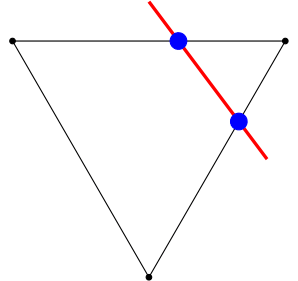
\includegraphics[width=0.3\textwidth]{FIG/TIKZ_LeftoverFigures_20230417/TIKZ_LeftoverFigures_20230417-1.png}
	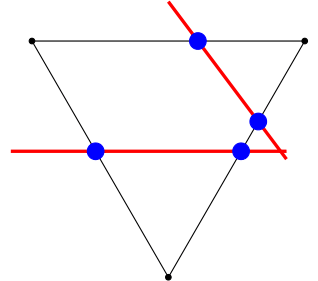
\includegraphics[width=0.3\textwidth]{FIG/TIKZ_LeftoverFigures_20230417/TIKZ_LeftoverFigures_20230417-2.png}
	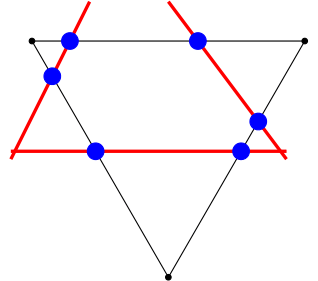
\includegraphics[width=0.3\textwidth]{FIG/TIKZ_LeftoverFigures_20230417/TIKZ_LeftoverFigures_20230417-3.png}
\end{center}
%\begin{center}
%	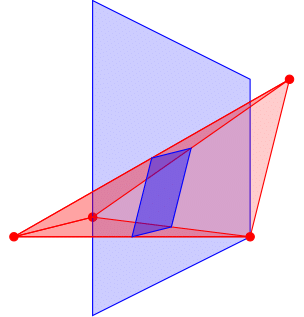
\includegraphics{FIG/TIKZ_LeftoverFigures_20230417/TIKZ_LeftoverFigures_20230417-4.png}
%	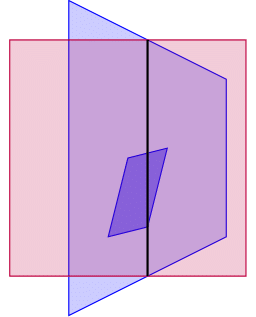
\includegraphics{FIG/TIKZ_LeftoverFigures_20230417/TIKZ_LeftoverFigures_20230417-5.png}
%\end{center}

A hyperplane divides vertices into two groups, one on each side.
We call the two groups \textbf{fathers and mothers}.
Any vertices lying directly on the hyperplane are grouped with the fathers.
\begin{center}
	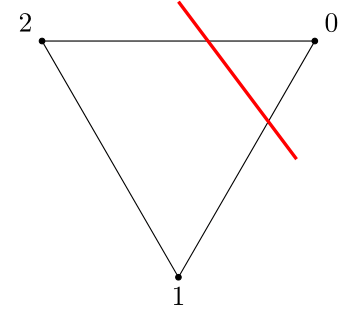
\includegraphics[width=0.45\textwidth]{FIG/TIKZ_SimplexFLAT_20230415/TIKZ_SimplexFlat_20230415-2.png}
	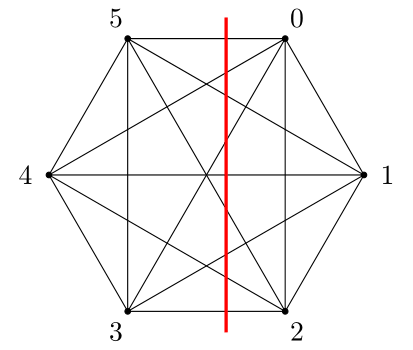
\includegraphics[width=0.45\textwidth]{FIG/TIKZ_SimplexFLAT_20230415/TIKZ_SimplexFlat_20230415-5.png}
\end{center}

A father and a mother with an edge between them create an intersection (\textbf{child}) with the hyperplane.
Not all fathers have children with all mothers, they must neighbour each other.
\begin{center}
	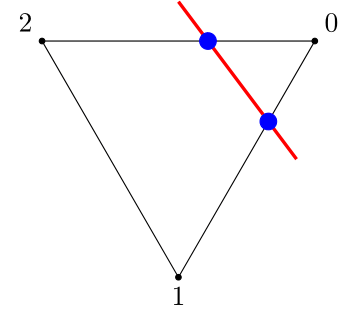
\includegraphics[width=0.45\textwidth]{FIG/TIKZ_SimplexFlat_20230415/TIKZ_SimplexFlat_20230415-3.png}
	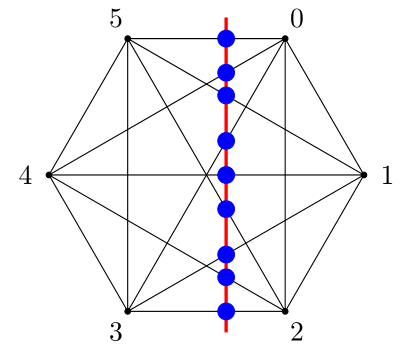
\includegraphics[width=0.45\textwidth]{FIG/TIKZ_SimplexFlat_20230415/TIKZ_SimplexFlat_20230415-6.png}
\end{center}
We need to be able to uniquely identify any intersection between simplex and hyperplane.
Let each vertex of the simplex have an \textbf{index} from 0 to $n$.
Then let the index of the child of any two parents be the \textbf{union of their indices}.
}

\headerbox{Siblings}{name=sib,column=1,row=0,span=1}{
Vertices of a section are the children of a father and a mother.
Two vertices are neighbours if their \textit{indices differ by exactly one element}.
Indices increase by one element after each sectioning.

If two children share a parent then their indices share the parent's index and differ by one element.
These children, called \textbf{siblings}, are therefore neighbours and have an edge between them.
}

\headerbox{Cross-hatching}{name=cross,column=1,row=0,span=1,below=sib}{
For each father, draw a vertical line.
For each mother, draw a horizontal line.
Every intersection is a child in the 1st order section.
\begin{center}
	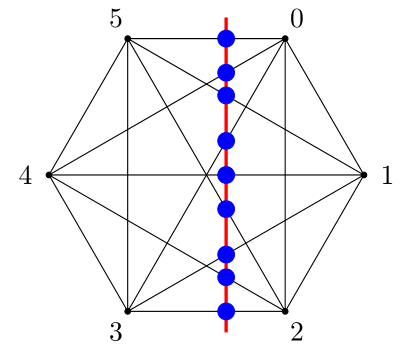
\includegraphics[width=0.45\textwidth]{FIG/TIKZ_SimplexFlat_20230415/TIKZ_SimplexFlat_20230415-6.png}
	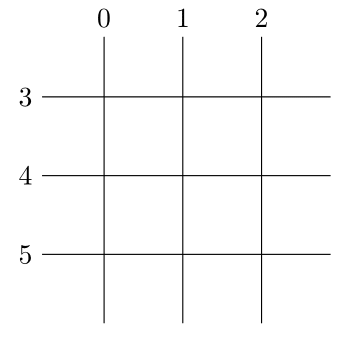
\includegraphics[width=0.45\textwidth]{FIG/TIKZ_Crosshatch_20230415/TIKZ_Crosshatch_20230415-2.png}
\end{center}
Any children connected along the same horizontal or vertical line of the cross-hatch are siblings.
This means each line represents a simplex.
This lets us draw the net of the section.
\begin{center}
	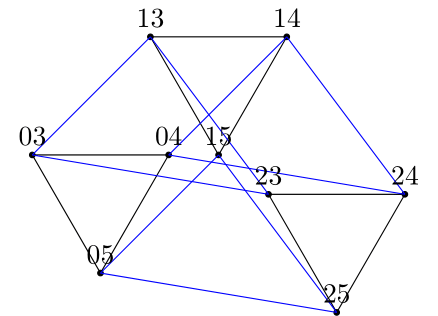
\includegraphics{FIG/TIKZ_NetSection_20230415/TIKZ_NetSection_20230415-2.png}
\end{center}
}

\headerbox{1st order sections}{name=1st,column=1,row=0,span=1,below=cross}{
\begin{lemma}
1st order sections are all duoprisms, the Cartesian product of two simplices.
\end{lemma}

\begin{proof}
Immediately follows from cross-hatching diagram.
\end{proof}
}

\headerbox{2nd order sections}{name=2nd,column=2,row=0,span=1}{
The vertices of the 1st order section are now parents for the 2nd order section.
Colour each child in the cross-hatch based on whether it is a father or a mother.
Since the section is convex, fathers and mothers are split into contiguous groups.
\begin{center}
	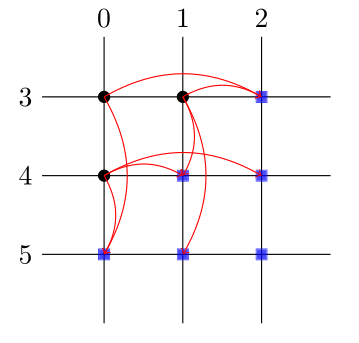
\includegraphics{FIG/TIKZ_Crosshatch_20230415/TIKZ_Crosshatch_20230415-3.png}
\end{center}

In the cross-hatch diagram, if one can draw a right-angled triangle with vertices a father and two mothers, or a mother and two fathers, then the two children associated with these parents are siblings.
Also, if three parents form a line, then their children are siblings.
\begin{center}
	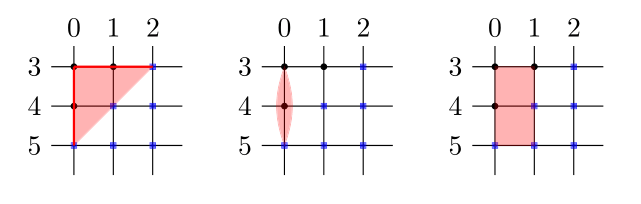
\includegraphics[width=\textwidth]{FIG/TIKZ_Crosshatch_20230415/TIKZ_Crosshatch_20230415-7.png}
\end{center}
If two children have fathers who are neighbours and mothers who are neighbours, then these chilrden (\textbf{cousins}) are neighbours in sections of order 2 and higher.
Only siblings and cousins are neighbours in 2nd order sections.
If one can draw a rectangle with vertices two fathers and two mothers, then the associated children are cousins.

We can draw the net, but it doesn't necessarily help us see the structure.
\begin{center}
	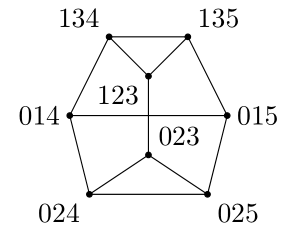
\includegraphics{FIG/TIKZ_NetSection_20230415/TIKZ_NetSection_20230415-3.png}
\end{center}
%Geometrically, this intersection cuts each cell (3D face) of the 1st order section with a plane.
%\begin{center}
%	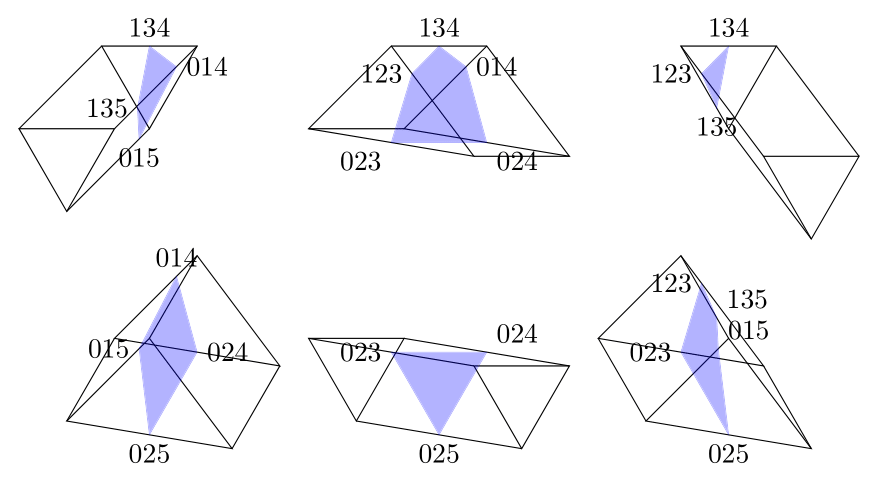
\includegraphics{FIG/TIKZ_NetSection_20230415/TIKZ_NetSection_20230415-4.png}
%\end{center}
}

\headerbox{General sections}{name=gen,column=3,row=0,span=1}{
\begin{lemma}
Vertices whose indices share all but $m$ elements all lie on the same $m$-face of the simplex.
\end{lemma}
\begin{center}
	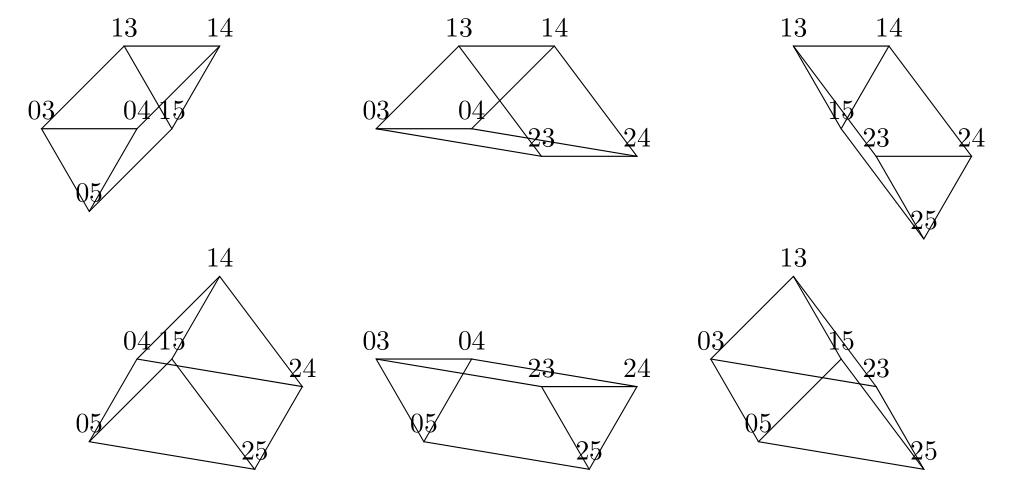
\includegraphics[width=\textwidth]{fig/TIKZ_NetSection_20230415/TIKZ_NetSection_20230415-5.png}
\end{center}

\begin{proof}
Each vertex in a $k$-th order section is the intersection of a $k$-dimensional face of the starting simplex and $k$ hyperplanes.
Suppose two vertices are indexed by sets $J$ and $K$ that share all but $m$ elements.
The set $J \cup K$ then has $k+m$ elements and indexes a $(k+m-1)$-dimensional face of the simplex, which is itself a simplex.
The section of this sub-simplex by the same $k$ hyperplanes that gave the original $k$-th order section gives an $m$-dimensional face of the original section.
Both $J$ and $K$ vertices lie on this face, since the $k$-dimensional faces of the starting simplex they index lie within the sub-simplex. % can this be turned into a proof by induction so that it's clearer?
\end{proof}

\begin{lemma}
Vertices of $k$-th order sections have exactly $n-k$ neighbours.
\end{lemma}

\begin{proof}
A $k$-th order section is a polytope in dimension $n-k$.
As such, each of its edges is shared with $n-k-1$ faces.
When taking the section of a $k$-th order section each edge cut by the hyperplane represents a child in the $(k+1)$-th order section.
Each face can be cut either twice or not at all, since the hyperplane restricted to the 2D subspace of the face is a line, giving two children per face.
By Lemma \ref{lem: faces} all indexing sets of the parents on the face share all but two indices, and so any children of the face share all but one element, making them neighbours.
This means each vertex of the $(k+1)$-th order section has $n-k-1$ neighbours.
\end{proof}
}

\headerbox{Conclusions}{name=conc,column=3,row=0,span=1,below=gen}{
Cross-hatching provides strategies for visualizing the intersection between simplices and hyperplanes.
This can help consider problems that might arise in algorithm design and geometric proofs.
}

\headerbox{References and links}{name=refs,column=0,row=1,span=1,below=sectioning}{
%nb: link to thesis? website?
}
 
\end{poster}

\end{document}